\section{Introduction}



In 2017,  \citet{oleson2017detecting} introduced a method for detecting time-specific differences in the trajectory of outcomes between experimental groups. Accompanying this was a novel method for controlling the family-wise error rate, particularly in the case of densely sampled time series where constructed test statistics exhibit high degrees of autocorrelation. This was followed up with in 2018 with the introduction of the \xt{bdots} package to CRAN \citep{seedorff2018bdots}. Here we reintroduce the \xt{bdots} package as a significant upgrade that broadly expands the capabilities of the original.
 

This manuscript is not intended to serve as a complete guide for using the \xt{bdots} package. Instead, the purpose is to showcase major changes and improvements, with those seeking a more comprehensive treatment directed to the package vignettes which are included in the appendix. Rather than taking a ``compare and contrast" approach, we will first enumerate the major changes, followed by a general demonstration of package use:

\begin{singlespace}
\begin{enumerate}
\item Major changes to underlying methodology with implications for prior users of the package
\item Simplified user interface
\item Introduction of user defined curves
\item Permit fitting for arbitrary number of groups
\item Automatic detection of paired tests based on subject identifier
\item Allows for non-homogeneous sampling of data across subjects and groups
\item Introduce formula syntax for bootstrapping difference function
\item Interactive refitting process
\end{enumerate}
\end{singlespace}


We start by clearly describing the type of problem that \xt{bdots} has been created to solve.

\paragraph{Bootstrapped differences in time series}

A typical problem in the analysis of differences in time series, and the kind that \xt{bdots} is intended to solve, involves that of two or more experimental groups containing subjects whose responses are measured over time. This may include the growth of tumors in  mice or the change in the proportion of fixations over time in the context of the VWP. In either case, we assume that each of the subjects $i = 1, \dots, n$  has observed data of the following form:

\begin{equation}\label{eq:mean_structure1}
y_{it} = f(t | \theta_i) + \epsilon_{it} 
\end{equation}
where $f$ represents a functional mean structure while the error structure of $\epsilon_{it}$ is open to being either IID or possess an AR(1) structure. At present, \xt{bdots} requires that each of the subjects being compared have the same parametric function $f$. This is not strictly necessary at the theoretical level, and future goals of the package include accommodating non-parametric functions. While the mean structures for each of the subjects is required to be of the same parametric form $f(\cdot | \theta)$, each differs in their instance of their own subject-specific parameters, $\theta_i$.

An explicit assumption of the current iteration of \xt{bdots} is that each subject $i$s' parameters within a group $g = 1, \dots, G$ is drawn from a group level distribution

\begin{equation}\label{eq:group_dist}
\theta_i \sim N(\mu_g, V_g).
\end{equation}

Bootstrapping these parameters gives an estimate of this distribution, which is then in turn used to construct a distribution of functions $f$. This in turn gives a representation of the temporal changes in group characteristics. It is precisely the identification of if and when these temporal changes differ between groups that \xt{bdots} seeks to accomplish.


\paragraph{Homogeneous Means Assumption}

The assumption presented in Equation~\ref{eq:group_dist} differs from the original iteration of \xt{bdots} in a critical way. In \citet{oleson2017detecting}, there was no assumption of variability between subject parameters, congruent with the assumption that $\theta_i = \theta_j$ for all subjects $i, j$ within a group. The most relevant consequence of the homogeneous means assumption is that there is no estimate of between-subject variability, resulting in a drastic inflation of the type I error. A detailed treatment of this issue and how it is resolved is handled in Chapter 4. For now, we will give a methodological overview of the process used by \xt{bdots} along with a presentation of an updated bootstrapping process and the introduction of a permutation test.




\section{Methodology and Overview} 

A standard analysis using \xt{bdots} consists of two steps: fitting the observed data to a specified parametric function, $f(\cdot|\theta)$, and then using the observed variability to construct estimates of the distributions of functions for groups whose differences we wish to investigate.  Here, we briefly detail how this is implemented in practice and introduce the new methodologies in \xt{bdots}. 



\subsection{Estimating Subject-Specific Curves}

We begin with the assumption that for subject $i$ in group $g$, we have collected observed data of the form given in Equation~\ref{eq:mean_structure1}, with the subject specific parameter $\theta_i$ following the distribution in Equation~\ref{eq:group_dist}. Each subject is then fit in \xt{bdots} via the nonlinear curve fitting function \xt{nlme::gnls}, returning for each set of observed data an estimated set of parameters $\hat{\theta}_i$ and their associated standard errors. From these estimates we are able to construct a sampling distribution for each subject:

\begin{equation}\label{eq:sub_dist}
\hat{\theta}_i \sim N(\theta_i, s_i^2).
\end{equation}

Just as in \citet{oleson2017detecting}, this distribution provides an estimate of the within-subject uncertainty in the estimate of subject-specific function parameters.




\subsection{Estimating Group Distributions}\label{sec:group_dist}

To help clarify the discussion that follows, we begin by reiterating a few important points. First, each subject that we consider in a \xt{bdots} analysis has a set of subject-specific parameters, $\theta_i$, which define the shape of their time series, itself assumed to be a parametric function. The collection of parameters of all subjects within a particular group make up a distribution of group parameters, the distribution given in Equation~\ref{eq:group_dist}. And although this distribution is specifically a distribution of \textit{parameters}, any sample of parameters from this distribution can be used to  construct a distribution of \textit{functions} that define a time series. In other words, we begin by observing a time series for each subject. We then fit parametric functions to these observed time series. These estimated parameters themselves make up a distribution of parameters. This distribution of parameters can then be used to construct a distribution of time series. 

In addition to the distribution of group parameters (Equation~\ref{eq:group_dist}), we have also described a distribution of subject-specific parameters (Equation~\ref{eq:sub_dist}). The motivation for the distribution given in Equation~\ref{eq:sub_dist} is as follows: for each individual subject, we wish to recover an estimate of the parameters that would be used to fit a parametric function to the observed time series data. In doing so, there is some degree of uncertainty that comes from the curve fitting process as evidenced by the standard errors. This accounts for within-subject variability. The insight of \citet{oleson2017detecting} was that this \textit{within-subject variability} should be accounted for when estimating the \textit{between-subject variability} present in the distribution of group parameters. That is, if each individual subjects' estimate was associated with a high degree of uncertainty, it would be appropriate for this uncertainty to be reflected in the total uncertainty representing the entire group.

With this in mind, we now propose the following algorithm for creating bootstrapped estimates of the \textit{group level distributions}:




\begin{enumerate}
\item For a group of size $n$, select $n$ subjects from the group \textit{with replacement}. This allows us to construct an estimate of $V_{g}$ from Equation~\ref{eq:group_dist}.
\item For each selected subject $i$ in bootstrap $b$, draw a set of parameters from the \textit{subject-specific} distribution 
\begin{equation}
\theta_{ib}^* \sim N(\hat{\theta}_i, s_i^2).
\end{equation}
\item Find the mean of each of the bootstrapped $\theta_{ib}^*$ in group $g$ to construct the $b$th group bootstrap, $\theta_{gb}^*$ where
\begin{equation}\label{eq:het_boot_dist}
\theta_{gb}^* = \frac1n \sum  \theta_{ib}^*, \qquad \theta_{gb}^* \sim N \left(\mu_g, \frac{1}{n} V_g + \frac{1}{n^2} \sum s_i^2 \right).
\end{equation}
That is, the bootstrapped estimate follows a \textit{group level} distribution
\item Perform steps (1)-(3) $B$ times, using each $\theta_{gb}^*$ to construct a sample of population curves, $f(\cdot| \mu_g)$.
\end{enumerate}

Note that the group level distribution in Equation~\ref{eq:het_boot_dist} differs from that under the homogeneous means assumption by the factor of $V_g$ in the variance term on account of the fact that subjects were originally sampled \emph{without} replacement


The final population curves from (4) can be used to create estimates of the mean response and an associated standard deviation at each time point for each of the groups bootstrapped. These estimates are used both for plotting and in the construction of confidence intervals. They also can be, but do not necessarily have to be, used to construct a test statistic, which is the topic of our next section.

\subsection{Hypothesis Testing  for Statistically Significant Differences in Time Series}

We now turn our attention to the primary goal of an analysis in \xt{bdots}, the identification of time windows in which the distribution of curves of two groups differ significantly. A problem unique to the ones addressed by \xt{bdots} is that of multiple testing; and especially in densely sampled time series, we must account for multiple testing while controlling the family-wise error rate (FWER). There are primarily two ways by which we are able to do this which we detail below.

\subsubsection{$\alpha$ Adjustment}

The first method whereby we control the FWER involves making adjustments to the nominal alpha value such as the case with a Bonferonni correction. Just as in the original iteration of \xt{bdots}, we are able to first construct test statistics from the bootstrapped estimates described in the previous section. These bootstrapped test statistics $T_t^{(b)}$ can be written as 

\begin{equation}\label{eq:test_statistic}
T_t^{(b)} = \frac{(\overline{p}_{1t} - \overline{p}_{2t})}{\sqrt{s_{1t}^2 + s_{2t}^2}},
\end{equation}
where $\overline{p}_{gt}$ and $s_{gt}^2$ are mean and standard deviation estimates  of the estimated functions at each time point $t$ and for groups $1$ and $2$, respectively. As was demonstrated in \cite{oleson2017detecting}, these test statistics can be highly correlated in the presence of densely sampled test statics, leading to an inflated type I error. The FWER in this case can be controlled with the adjustment proposed in \citet{oleson2017detecting}. In addition to this, adjustments to the nominal alpha can also be made using all of the adjustments present in \xt{p.adjust} from the R \xt{stats} package.


\subsubsection{Permutation Testing}

In addition to modified correction based on the bootstrapped test statistics, \xt{bdots} provides a permutation test for controlling the FWER without any additional assumptions of autocorrelation. 

In doing so, we begin by creating an observed test statistic in the following way: first, taking each subject's estimated parameter $\hat{\theta}_i$, we find the subject's corresponding parametric curve $f(t|\hat{\theta}_i)$. Within each group, we use \textit{these} curves to create estimates of the mean population curves and associated standard errors at each point\footnote{This differs from the bootstrapped test statistic in which the mean of the subjects' parameters was used to fit a population curve, i.e., $\frac1n \sum f(t|\theta_i)$ compared with $f \left( t | \frac1n \sum \theta_i \right)$. The implications of this have not been investigated any further}. Letting $p_{gt}$ and $s_{gt}^2$ represent the mean population curve and standard error for group $g$ at time $t$, we define our observed permutation test statistic, 

\begin{equation}\label{eq:perm_stat}
T_t^{(p)} = \frac{|\overline{p}_{1t} - \overline{p}_{2t}|}{\sqrt{s_{1t}^2 + s_{2t}^2}}.
\end{equation}.

We then going about using permutations to construct a null distribution against which to compare the observed statistics from Equation~\ref{eq:perm_stat}. We do so with the following algorithm:

\begin{enumerate}
\item Assign to each subject a label indicating group membership
\item Randomly shuffle the labels assigned in (1.), creating two new groups 
\item Recalculate the test statistic $T^{(p)}_t$, recording the maximum value from each permutation
\item Repeat (2.)-(3.) $P$ times. The collection of $P$ statistics will serve as our null distribution, denoted $\widetilde{T}$. Let $\widetilde{T}_{\alpha}$ be the $1 - \alpha$ quantile of $\widetilde{T}$. Areas where the observed $T^{(p)}_t > \widetilde{T}_{\alpha}$ are designated significant.
\end{enumerate}

Paired statistics can also be constructed in both the bootstrap and permutation methods. This is implemented by ensuring that at each bootstrap the same subjects are selected for each group or by ensuring that each permuted group contains one observation from each subject.

A demonstration of power and FWER control for both the heterogeneous bootstrap and permutation test are given in Chapter 4.


In the following sections, we detail the two major components of an analysis using the \xt{bdots} package, curve fitting and the identification of statistically significant differences in time series. Within each section, we will begin with a high level explanation of the major changes that have been made, along with a detailed description of the function syntax. We then concretize this discussion with a real world example along with illustrations of function calls and return objects.


\section{Curve Fitting}

The first step in performing an analysis with \xt{bdots} involves specifying the parametric function which defines the mean structure from Equation~\ref{eq:mean_structure1} and fitting curves to the observed data for each subject. Throughout this discussion and into the next section, we will use as our real world example a comparison of tumor growth for the 451LuBr cell line in mice with repeated measures across five treatment groups. A depiction of this data is given in Figure~\ref{fig:mouse_head}.

\begin{singlespace}
\begin{figure}[H]
\centering
\begin{BVerbatim}
> head(mouse, n = 10)
      Volume Day Treatment ID
 1:   47.432   0         A  1
 2:   98.315   5         A  1
 3:  593.028  15         A  1
 4:  565.000  19         A  1
 5: 1041.880  26         A  1
 6: 1555.200  30         A  1
 7:   36.000   0         B  2
 8:   34.222   4         B  2
 9:   45.600  10         B  2
10:   87.500  16         B  2
\end{BVerbatim}
\caption{Illustration of Mouse data in long format}
\label{fig:mouse_head}
\end{figure}
\end{singlespace}

A new feature of \xt{bdots} is the ability to fit and analyze subjects with non-homogeneous time samples, which we see in the \xt{Day} variable values in the mouse data in Figure~\ref{fig:mouse_head}. 

A new feature of \xt{bdots} is the ability to fit and analyze subjects with non-homogeneous time samples. For example, consider the \xt{Day} column for our mouse data shown in Figure~\ref{fig:mouse_head}, where the first four observations for ID 1 are all different than those for ID 2. For the present analysis, we will be interested in determining if and when the trajectory of tumor growth (measured in volume) changes between any two treatment groups.


There are two primary functions in the \xt{bdots} package: one for fitting the observed data to a parametric function and another for estimating group distributions and identifying time windows where they differ significantly. The first of these, \xt{bfit}, is the topic of this section.


\paragraph{The \xt{bfit} Function}

The curve fitting process is performed with the function \texttt{bfit} , taking the following arguments:


\begin{figure}[h!]
\centering
\begin{BVerbatim}
bfit(data, subject, time, y, group, curveType, ar, ...)
\end{BVerbatim}
\caption{Main arguments to \xt{bfit}, though see \xt{help(bfit)} for additional options}
\end{figure}



The \xt{data} argument takes the name of the dataset being used. \xt{subject} is the subject identifier column in the data and should be passed as a character. It is important to note here that the identification of paired data is now done automatically; in determining if two experimental groups are paired, \xt{bdots} checks that the intersection of subjects in each of the groups are identical with the subjects in each of the groups individually. As such, it will be important for the user to be sure that if the data is paired that the subject identifiers are the same between subject groups. 

The \xt{time} and \xt{y} arguments are column names of the time variable and outcome, respectively. Similarly, \xt{group} takes as an argument a character vector of each of the group columns that are meant to be fit, accommodating the fact that \xt{bdots} is now able to fit an arbitrary number of groups at once provided that the outcomes in each group adopt the same parametric form. And lastly, the \xt{curveType} argument, which is used to specify details of the parametric function to which the data will be fit. As this argument is more involved, we will address it separately in the next section.



\paragraph{\xt{curveType} functions} Whereas the previous iteration of \xt{bdots} had a separate fitting function for each parametric form (i.e., \xt{logistic.fit} for fitting data to a four-parameter logistic), we are now able to specify the curves we wish to fit independent of the fitting function, passed as an argument to \xt{bfit}. This is done with the argument \xt{curveType}. Unlike the previous arguments which took either a \xt{data.frame} or character  vector, \xt{curveType} takes as an argument a function call, for example, \xt{logistic()}. In short, this allows the user to pass additional arguments to further specify the curve. For example, among the parametric functions now included in \xt{bdots} is the \xt{polynomial} function, taking as an additional argument the number of degrees we wish to use. To fit the observed data with a five parameter polynomial in \xt{bfit}, one would then pass the argument \xt{curveType = polynomial(degree = 5)}. Curve functions currently included in \xt{bdots} are \xt{logistic()}, \xt{doubleGauss()}, \xt{expCurve()}, and \xt{polynomial()}. In addition to the functions provided by default in the \xt{bdots} package, \xt{bfit} can also accept user-created curves; a detailed explanation of how this is done is provided in the appendix as well as with \xt{vignette("bdots")}.

Using our mouse data with the columns shown in Figure~\ref{fig:mouse_head}, we are ready to fit curves to each of the subjects. For this analysis we will fit data to an exponential curve of the form
\begin{equation}
f(t|\theta) = x_0 e^{tk}
\end{equation}
where $\theta = [x_0, k]$. This form is specified in the \xt{expCurve()} provided by the \xt{bdots} package.


\begin{singlespace}
\begin{figure}[H]
\centering
\begin{BVerbatim}
mouse_fit <- bfit(data = mouse, subject = "ID", time = "Day", 
                  y = "Volume", group = "Treatment", curveType = expCurve())
\end{BVerbatim}
%\caption{Fitting mouse data with \xt{bfit} -- should I caption these?}
\label{fig:bfit_example}
\end{figure}
\end{singlespace}

Having successfully fit curves to our data, we now consider the return object and provided summaries. 


\paragraph{Return Object and Generics}

The function \xt{bfit} returns an object of class \xt{bdotsObj}, inheriting from class \xt{data.table}. As such, each row uniquely identifies one combination of subject and group values. Included in this row are the subject identifier, group classification, summary statistics regarding the curves, and a nested \xt{gnls} object. Inheriting from \xt{data.table} also permits us to use \xt{data.table} syntax to subset the object as in Figure~\ref{fig:plot_fits}  where we elect to only plot the first four subjects.

\begin{singlespace}
\begin{figure}[H]
\centering
\begin{BVerbatim}
> class(mouse_fit)
[1] "bdotsObj"   "data.table" "data.frame"

> head(mouse_fit)
   ID Treatment        fit      R2   AR1 fitCode
1:  1         A <gnls[18]> 0.97349 FALSE       3
2:  2         B <gnls[18]> 0.83620 FALSE       4
3:  3         E <gnls[18]> 0.96249 FALSE       3
4:  4         C <gnls[18]> 0.96720 FALSE       3
5:  5         D <gnls[18]> 0.76156 FALSE       5
6:  7         B <gnls[18]> 0.96361 FALSE       3
\end{BVerbatim}
\caption{A \xt{bfit} object inheriting from \xt{data.frame}}
\label{fig:bdotsObj}
\end{figure}
\end{singlespace}

The number of columns will depend on the total number of groups specified, with the subject and group identifiers always being the first columns. Following this is the \xt{fit} column, which contains the fitted object returned from \xt{gnls}, as well as \xt{R2} indicating the $R^2$ statistic. The \xt{AR1} column indicates whether or not the observed data was able to be fit with an AR(1) error assumption. Finally, there is the \xt{fitCode} column, which provides a numerical summary on the quality of fits.

Several methods exist for this object, including \xt{plot}, \xt{summary}, and \xt{coef}, returning a matrix of fitted coefficients obtained from \xt{gnls}. 


\paragraph{Fitting Diagnostics}\label{sec:fitcode}

The \xt{bdots} package was originally introduced to address a very narrow scope of problems, and the \xt{fitCode} designation is an artifact of this original intent. Specifically, it assumed that all of the observed data was of the form given in Equation~\ref{eq:mean_structure1} where the observed time series was dense and the errors were autocorrelated. Autocorrelated errors can be specified in the \xt{gnls} package (used internally by \xt{bdots}) when generating subject fits, though there were times when the fitter would be incapable of converging on a solution. In that instance, the autocorrelation assumption was dropped and constructing a fit was reattempted.

$R^2$ proved a reliable metric for this kind of data, and preference was given to fits with an autocorrelated error structure over those without. From this, the hierarchy given in Table~\ref{tab:fit_codes} was born. \xt{fitCode} is a numeric summary statistic ranked from 0 to 6 detailing information about the quality of the fitted curve, constructed with the following pseudo-code:

\begin{singlespace}
\begin{figure}[H]
\centering
\begin{BVerbatim}
  AR1 <- # boolean, determines AR1 status of fit
  fitCode <- 3*(!AR1) + 1*(R2 < 0.95)*(R2 > 0.8) + 2*(R2 < 0.8)
\end{BVerbatim}
%\caption{Illustration of Mouse data}
\end{figure}
\end{singlespace}

A fit code of 6 indicates that \xt{gnls} was unable to successfully fit the 
subject's data. 

\xt{bdots} today stands to accommodate a far broader range of data for which the original \xt{fitCode} standard may no longer be relevant. The presence of autocorrelation cannot always be assumed, and users may opt for a metric other than $R^2$ for assessing the quality of the fits. Even the assessments of fits on a discretized scale may be something of only passing interest. Even then, however, this is how the current implementation of \xt{bdots} categorizes the quality of its fits, with the creation of greater flexibility in this regard being a priority for future directions. 

\begin{singlespace}
\begin{table}[H]
\centering
\def\arraystretch{1.5}
\begin{tabular}{|c|c|c|}
\hline
\xt{fitCode} & AR(1) & $R^2$ \\
\hline
0 & TRUE & $R^2 > 0.95$ \\
1 & TRUE & $0.8 < R^2 < 0.95$ \\
2 & TRUE & $ R^2 <0.8$ \\
3 & FALSE & $R^2 >0.95$ \\
4 & FALSE & $0.8 < R^2 < 0.95$ \\
5 & FALSE &$ R^2 <0.8$  \\
6 & NA & NA \\
\hline
\end{tabular}
\caption{Description of the \xt{fitCode} statistic}
\label{tab:fit_codes}
\end{table}
\end{singlespace}

While the fit code offers a simple diagnostic for assessing quality of individual subjects, it will often be useful to consider broader summaries for reporting on the quality of fits for groups as a whole. This is done most simply using the \xt{summary} and \xt{plot} functions. 


\paragraph{Summaries and Plots}

Users are able to quickly summarize the quality of the fits with the \xt{summary} method now provided. For example, we may consider a summary of the fitted mouse data:

\begin{singlespace}
\begin{figure}[H]
\centering
\begin{BVerbatim}
> summary(mouse_fit)

bdotsFit Summary

Curve Type: expCurve 
Formula: Volume ~ x0 * exp(Day * k) 
Time Range: (0, 106) [31 points]

Treatment: A 
Num Obs:  10 
Parameter Values: 
        x0          k 
172.232953   0.056843 
########################################
############### FITS ###################
########################################
AR1,       0.95 <= R2        -- 2 
AR1,       0.80 < R2 <= 0.95 -- 1 
AR1,       R2 < 0.8          -- 0 
Non-AR1,   0.95 <= R2        -- 0 
Non-AR1,   0.8 < R2 <= 0.95  -- 3 
Non-AR1,   R2 < 0.8          -- 4 
No Fit                       -- 0 

[...]

All Fits 
Num Obs:  42 
Parameter Values: 
        x0          k 
102.487118   0.053662 
########################################
############### FITS ###################
########################################
AR1,       0.95 <= R2        -- 4 
AR1,       0.80 < R2 <= 0.95 -- 2 
AR1,       R2 < 0.8          -- 0 
Non-AR1,   0.95 <= R2        -- 9 
Non-AR1,   0.8 < R2 <= 0.95  -- 16 
Non-AR1,   R2 < 0.8          -- 11 
No Fit                       -- 0 
\end{BVerbatim}
\caption{Abridged output from the summary function. Note that this includes data on the formula used, the quality of fits and mean parameter estimates by group, and a summary of all fits combined}
\end{figure}
\end{singlespace}

It is also recommended that users visually inspect the quality of fits for their subjects, which includes a plot of both the observed and fit data. There are a number of options available in \xt{?plot.bdotsObj}, including the option to fit the plots in base R rather than \xt{ggplot2}. This is especially helpful when looking to quickly assess the quality of fits as \xt{ggplot2} can be notoriously slow with large data sets. Figure~\ref{fig:plot_fits} includes a plot of the first four fitted subjects.


\begin{singlespace}
\begin{figure}[H]
\centering
\begin{BVerbatim}
plot(mouse_fit[1:4, ])
\end{BVerbatim}
\end{figure}
\end{singlespace}

\begin{figure}[H]
\centering
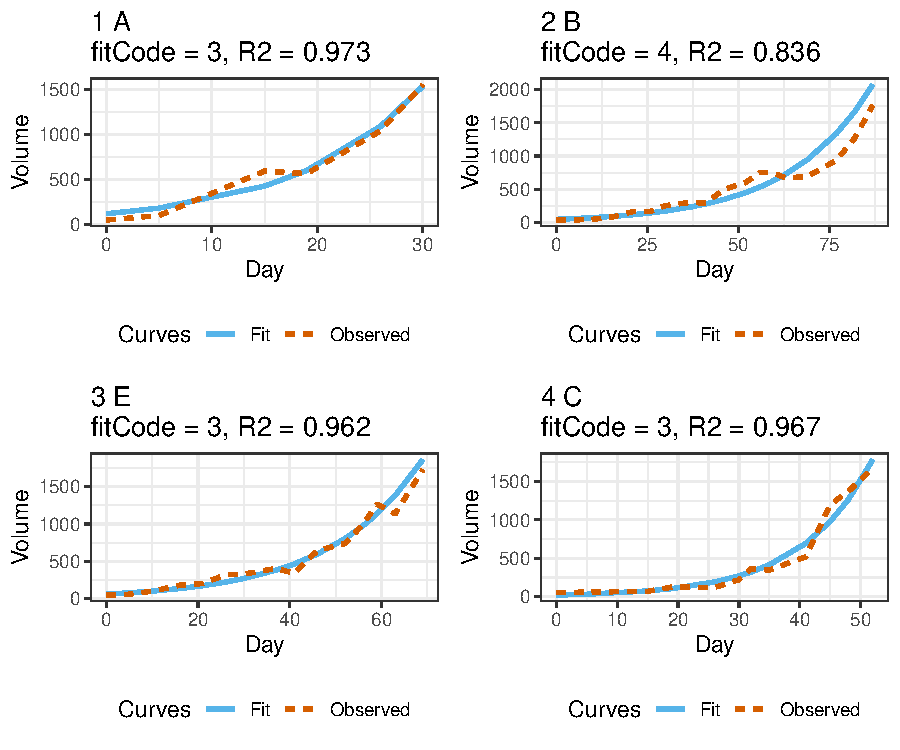
\includegraphics[width=0.9\textwidth]{img/mouse_fit.pdf}
\caption{Plot of \xt{mouse\_fit} using  \xt{data.table} syntax to subset to only the first four observations}
\label{fig:plot_fits}
\end{figure}

\xt{bdots} provides now an interactive refitting function, \xt{brefit}, which provides a number of options to help users recalibrate low quality fits. Details on this function and how it is used are provided in Section~\ref{sec:anc_func}.


\section{Identification of Group Differences}

Having satisfactorily fit subject-specific parametric curves to the observed data, we are ready to begin estimating the group distributions and investigating temporal differences. This section details the function for doing so, \xt{bboot}, along with the introduction of a formula syntax that is new and unique to \xt{bdots}. As before, we will follow each of our descriptions with an illustration of use with the mouse tumor data. Following this, we summarize new generics that are available to the object returned by \xt{bboot}, including those for the \xt{summary} and \xt{plot} functions.


\paragraph{The \xt{bboot} Function}

This is done with the bootstrapping\footnote{Although both bootstrapping and permutation testing are available for statistically testing temporal differences, bootstrapping is still used for the construction of confidences intervals given in the \xt{plot} function, hence the description as a ``bootstrapping" function} function, \xt{bboot}. The number of options included in the \xt{bboot} function have expanded to include a new formula syntax for specifying the analysis of interest as well as to include options for permutation testing. A call to \xt{bboot} takes the following form:

\begin{singlespace}
\begin{figure}[H]
\centering
\begin{BVerbatim}
bboot(formula, bdObj, B, alpha, permutation = TRUE, padj = "oleson", ...)
\end{BVerbatim}

\end{figure}
\end{singlespace}

The \xt{formula} argument is new to  \xt{bdots} and will be discussed in the next section. As for the remaining arguments, \xt{bdObj} is simply the object returned from \xt{bfit} that we wish to investigate, and \xt{B} serves the dual role of indicating the number of bootstraps/permutations we wish to perform; \xt{alpha} is the rate at which we wish to control the FWER. \xt{permutation} and \xt{padj} work in contrast to one another: when \xt{permutation = TRUE}, the argument to \xt{padj} is ignored. Otherwise, \xt{padj} indicates the method to be used in adjusting the nominal \xt{alpha} to control the FWER. By default, \xt{padj = "oleson"}. Finally, as previously mentioned, there is no longer a need to specify if the groups are paired, and \xt{bboot} determines this automatically based on the subject identifiers in each of the groups.


\paragraph{Formula} \label{sec:formula}

As the \xt{bfit} function is now able to create fits for an arbitrary number of groups at once, we rely on a formula syntax in \xt{bboot} to specify precisely which groups differences we wish to compare. Let \xt{y} designate the outcome variable indicated in the \xt{bfit} function and let \xt{group} be one of the group column names to which our functions were fit. Further, let \xt{val1} and \xt{val2} be two values within the \xt{group} column. The general syntax for the \xt{bboot} function takes the following form:


\begin{center}
\tt y $\sim$ group(val1, val2)
\end{center}

Note that this is an \textit{expression} in R and is written without quotation marks. To give a more concrete example, suppose we wished to compare the difference in tumor growth curves for A and B from the \xt{Treatment} column in our mouse data (Figure~\ref{fig:mouse_head}). We would do so with the following syntax:


\begin{center}
\tt Volume $\sim$ Treatment(A, B)
\end{center}

\cn{I still think the extended formula syntax belongs in the appendix. It is completely out of left fucking field to bring in a car example here, and the mouse data does not naturally accommodate anything we wish to detail}

There are two special cases to consider when writing this syntax. The first is the situation that arises in the case of multiple or nested groups, the second when a difference of difference analysis is conducted. We will describe these in the next section, though it is important to note here that the mouse data being used to provide illustration to the package use does not naturally accommodate either of these extensions. As such, we will begin by briefly introducing a mock data structure and then using it to illustrate the extensions of the syntax.


\paragraph{Formula Syntax for Nested Groups and the Difference of Differences} 

The formula syntax introduced in Section \ref{sec:formula} is straightforward enough in the case in which we are interested in comparing two groups within a single category, as is the case when we compare two treatment groups, both within the \xt{Treatment} column. As \xt{bdots} now allows multiple groups to be fit at once, there may be situations in which we need more precision in specifying what exactly we wish to compare. Consider for example an artificial dataset that contains some outcome \xt{y} for a collection of vehicles, consisting of eight distinct groups, nested in order of vehicle origin (foreign or domestic), vehicle class (car or truck), and vehicle color (red or blue). A table detailing the relationship of the groups is given in Table~\ref{tab:vehicle}.

\begin{table}[H]
\centering
\def\arraystretch{1.5}
\begin{tabular}{|p{0.9in}|p{0.9in}|p{0.9in}|} \hline 
\rowcolor{lightgray} \multicolumn{1}{|c|}{Origin} & \multicolumn{1}{c|}{Class} & \multicolumn{1}{c|}{Color}\\
\hline
\multirow{4}{*}{foreign} & \multirow{2}{*}{car} & red \\
\hhline{~~-}
& & blue \\
\hhline{~--}
& \multirow{2}{*}{truck} & red \\
\hhline{~~-}
& & blue \\
\hline
\multirow{4}{*}{domestic} & \multirow{2}{*}{car} & red \\
\hhline{~~-}
& & blue \\
\hhline{~--}
& \multirow{2}{*}{truck} & red \\
\hhline{~~-}
& & blue \\
\hline
\end{tabular}
\caption{Example of nested vehicle classes}
\label{tab:vehicle}
\end{table}


Beginning with a simple case, suppose we want to investigate the difference in outcome between all foreign and domestic vehicles. Notionally, we would write

\begin{center}
\tt y $\sim$ Origin(foreign, domestic)
\end{center}
just as we did in the mouse data example: here, the name of the group variable \xt{Origin}, followed by the values we are interested in comparing, \xt{domestic} and \xt{foreign}. Alternatively, if we wanted to limit our investigation to only foreign and domestic \textit{trucks}, we would do this by including an extra term specifying the group and the desired value. In this case:

\begin{center}
\tt y $\sim$ Origin(foreign, domestic) + Class(truck).
\end{center}

Similarly, to compare only foreign and domestic \textit{red} trucks, we would add an additional term for color:

\begin{center}
\tt y $\sim$ Origin(foreign, domestic) + Class(truck) + Color(red)
\end{center}

There are also instances in which we might be considered in the interaction between two groups. Although there is no native way to handle interactions in \xt{bdots}, this can be done indirectly through the difference of differences \citep{McMurray2019}. To illustrate, suppose we are interested in understanding how the color of the vehicle differentially impacts outcome based on the vehicle class. In such a case, we might look at the difference in outcome between red cars and red trucks and then compare this against the difference between blue cars and blue trucks. Any difference between these two differences would give information regarding the differential impact of color between each of the two classes. This is done in \xt{bdots} using the \xt{diffs} syntax in the formula:

%\textbf{FOUND SOURCE FOR THIS:} \textit{McMurray, Klein-Packard, Tomblin 2019, real time mechanics..pg 7}

\begin{center}
\tt diffs(y, Class(car, truck)) $\sim$ Color(red, blue)
\end{center}

Here, the \textit{outcome} that we are considering is the difference between vehicle classes, with the groups we are interested in comparing being color. This is helpful in remembering which term goes on the left hand side of the formula. 

Similar as to the case before, if we wanted to limit this difference of differences investigation to only include domestic vehicles, we can do so by including an additional term:

\begin{center}
\tt diffs(y, Class(car, truck)) $\sim$ Color(red, blue) + Origin(domestic).
\end{center}

As before, this can be further subset with an arbitrary number of nested groups.

We now return to a description of the process of estimating group differences with the mouse tumor dataset.


\paragraph{Summary and Analysis}

Let's begin first by running \xt{bboot} using bootstrapping to compare the difference in tumor growth between treatment groups A and E in our mouse data using permutations to test for regions of significant difference. 


\begin{center}
\tt mouse\_boot <- bboot(Volume $\sim$ Treatment(A, E), bdObj = mouse\_fit, permutation = TRUE)
\end{center}


This returns an object of class \xt{bdotsBootObj}. A summary method is included to display relevant information:

\begin{singlespace}
\begin{figure}[H]
\centering
\begin{BVerbatim}
> summary(mouse_boot)

bdotsBoot Summary

Curve Type: expCurve 
Formula: Volume ~ x0 * exp(Day * k) 
Time Range: (0, 59) [21 points]

Difference of difference: FALSE 
Paired t-test: FALSE 
Difference: Treatment 

FWER adjust method: Permutation 
Alpha: 0.05 
Significant Intervals:
     [,1] [,2]
[1,]   15   32
\end{BVerbatim}
%\caption{Illustration of Mouse data}
\end{figure}
\end{singlespace}

There are a few components of the summary that are worth identifying when reporting the results. In particular, note the time range provided, an indicator of if the test was paired, and which groups were being considered. The last section of the summary indicates the testing method used, an adjusted \xt{alphastar} if \xt{permutation = FALSE}, and a matrix of regions identified as being significantly different. This matrix is \xt{NULL} is no differences were identified at the specified alpha; otherwise there is one row included for each disjointed region of significant difference.

In addition to the provided summary output, a \xt{plot} method is available, with a list of additional options included in \xt{help(plot.bdotsBootObj)}.

\begin{figure}[H]
\centering
\begin{BVerbatim}
plot(mouse_boot)
\end{BVerbatim}

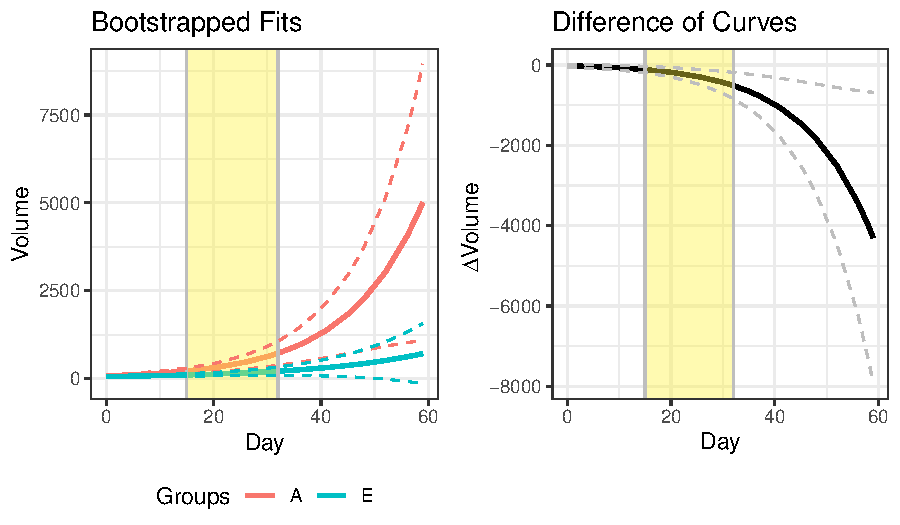
\includegraphics{img/mouse_boot_plot.pdf}
\caption{Bootstrapped distributions with regions of significant difference determined via permutation testing}
\end{figure}
%
%Depending on user needs, these plots can be recreated both without confidence bands or without the additional difference curve
%
%\begin{figure}[H]
%\centering
%\begin{BVerbatim}
%plot(mouse_boot, ciBands = FALSE, plotDiffs = FALSE)
%
%\end{BVerbatim}
%
%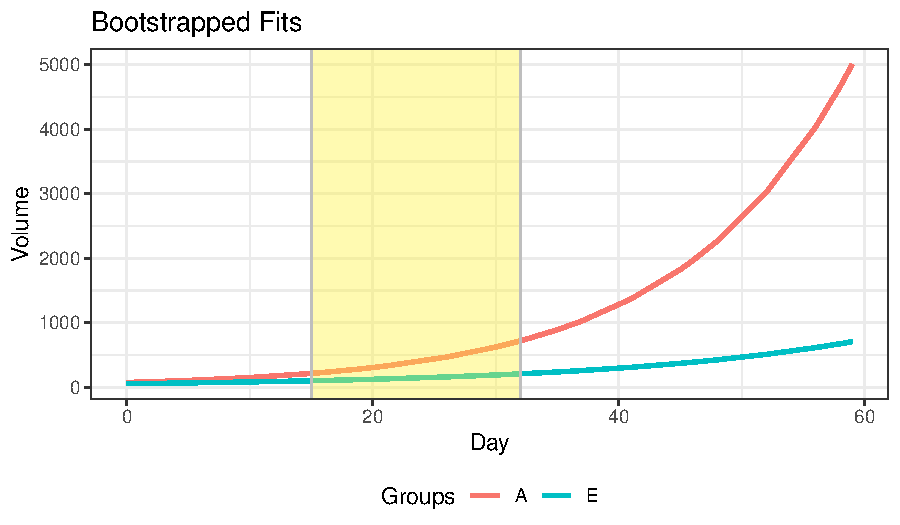
\includegraphics{img/mouse_boot_plot_extra.pdf}
%\caption{I think I'm going to actually not include this}
%\end{figure}


\section{Ancillary Functions}\label{sec:anc_func}

Outside of a standard analysis using the \xt{bdots} package, there are a suite of functions that users may find helpful. Brief descriptions of these additional functions are given here. 


\subsection{Refitting}

The nonlinear curve fitting algorithm used by \xt{nlme::gnls} in \xt{bfit} can be sensitive to the starting parameters. Sensible starting parameters are computed from the observed data as part of the curve fitting functions (i.e., within the \xt{logistic()} function), though these can often be improved upon. The quality of the fits can often be evidenced by the \xt{fitCode} or via  visual inspections of the fitted functions against the observed data. There are sometimes, however, when the quality of fits are poor. When this occurs, there are several options available to the user, all of which are provided through the function \xt{brefit}. \xt{brefit} takes the following arguments:

\begin{singlespace}
\begin{figure}[H]
\centering
\begin{BVerbatim}
brefit(bdObj, fitCode = 1L, subset = NULL, quickRefit = FALSE, paramDT = NULL)
\end{BVerbatim}
%\caption{Illustration of Mouse data}
\end{figure}
\end{singlespace}

The first of these arguments outside of the \xt{bdObj} is \xt{fitCode}, indicating the minimum fit code to be included in the refitting process. As discussed in Section~\ref{sec:fitcode}, this can be a sub-optimal way to specify data to subset. To add flexibility to which subjects are fit there is now the \xt{subset} argument taking either a logical expression, a collection of indices that would be used to subset an object of class \xt{data.table}, or a numeric vector with indices that the user wishes to refit. For example, we could elect to refit only the first 10 subjects or refit subjects with $R^2 < 0.9$:

\begin{singlespace}
\begin{figure}[H]
\centering
\begin{BVerbatim}
refit <- brefit(fit, subset = 1:10) # refit the first 10 subjects
refit <- brefit(fit, subset = R2 < 0.9) # refit subjects with R2 < 0.9
\end{BVerbatim}
%\caption{Illustration of Mouse data}
\end{figure}
\end{singlespace}

When an argument is passed to subset, the \xt{fitCode} argument is completely ignored.

To assist with the refitting process is the argument \xt{quickRefit}. When set to \xt{TRUE}, \xt{brefit} will take the average coefficients of accepted fits within a group and use those as new starting parameters for poor fits. The new fits will be retained if they have a larger $R^2$ value by default. When set to \xt{quickRefit = FALSE}, the user will be guided through a set of prompts to refit each of the curves manually. 

Finally, the \xt{paramDT} argument allows for a \xt{data.table} with columns for subject, group identifiers, and parameters to be passed in as a new set of starting parameters. This \xt{data.table} requires the same format as that returned by \xt{bdots::coefWriteout}. The use of this functionality is covered in more detail in the \xt{bdots} vignettes and is a useful way for reproducing a \xt{bdotsObj} from a plain text file. 

When \xt{quickRefit = FALSE}, the user is put through a series of prompts along with a series of diagnostics for each of the subjects to be refit. Here, for example, is the option to refit subject 11 from the mouse data:


\begin{singlespace}
\begin{figure}[H]
\centering
\begin{BVerbatim}
Subject: 11
R2: 0.837
AR1: FALSE
rho: 0.9
fitCode: 4

 Model Parameters:
       x0         k 
53.186497  0.051749 

Actions:
1) Keep original fit
2) Jitter parameters
3) Adjust starting parameters manually
4) Remove AR1 assumption
5) See original fit metrics
6) Delete subject
99) Save and exit refitter
Choose (1-6):
\end{BVerbatim}
%\caption{Illustration of Mouse data}
\end{figure}
\end{singlespace}

There are a number of options provided in this list. The first, of course, keeps the original fit of the presented subject and moves on to the next subject in the list. The second option takes the values of the fitted parameter and ``jitters" them, changing each of the values by a prespecified magnitude. Given the sensitivity of \xt{nlme::gnls} to starting parameters, this is sometimes enough for the fitter to converge on a better fit for the observed data. Alternatively, the third option gives the user the ability to select the starting parameters manually. The third option gives the user the ability to attempt refitting the observed data without an AR(1) error assumption, though this is only relevant if such an assumption exists. Option (5) reprints summary information and option (6) allows the user to delete the subject all together.

When any attempt to refit the observed under new conditions is presented (options (2)-(4)), a plot is rendered comparing the original fit side-by-side with the new alternative, Figure~\ref{fig:refit_plot}.

\begin{figure}[H]
\centering
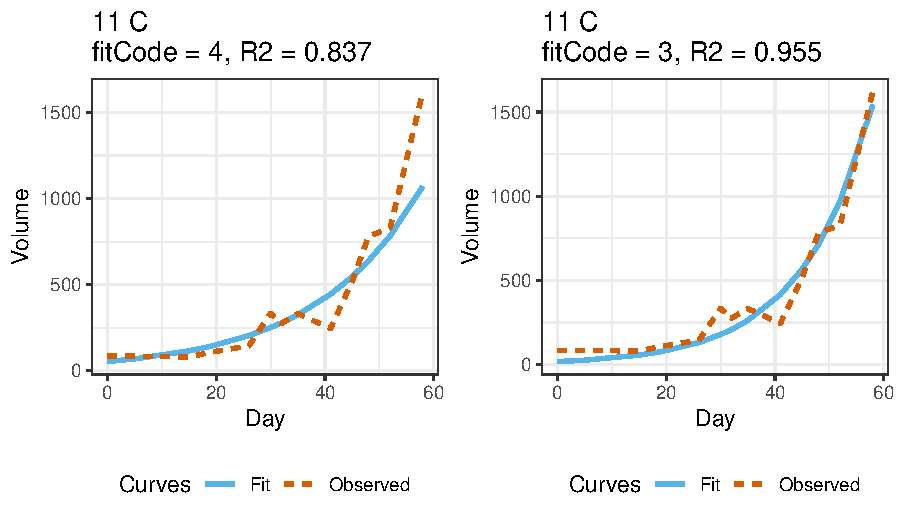
\includegraphics{img/mouse_refit_plot.pdf}
% new pars x0=50, k = 0.06
\caption{before and after refit}
\label{fig:refit_plot}
\end{figure}

As the menu item suggests, users have the ability to end the manually refitting process early and save where they had left off. To retain previously refit items and start again at a later time, pass the first refitted object back into the refitter as such:

\begin{singlespace}
\begin{figure}[H]
\centering
\begin{BVerbatim}
refit <- brefit(fit, ...)
refit <- brefit(refit, ...) # pass in the refitted object
\end{BVerbatim}
%\caption{Illustration of Mouse data}
\end{figure}
\end{singlespace}



A final note should be said regarding the option to delete a subject. As \xt{bdots} now automatically determines if subjects are paired based on subject identifiers (necessary for  calculations in significance testing), it is critical that if a subject has a poor fit in one group and must be removed that they are also removed from all additional groups in order to retain paired status. This can be overwritten with a final prompt in the \xt{brefit} function before they are removed. The removal of subjects can also be done with the ancillary function, \xt{bdRemove}, useful for removing subjects without undergoing the entire refitting process. See \xt{help(bdRemove)} for details.


\subsection{Correlations}

There are sometimes cases in which we are interested in determining the correlation of a fixed attribute with group outcome responses across time . This can be done with the \xt{bcorr} function (previously \xt{bdotsCorr}), which takes as an argument an object of class \xt{bdotsObj} as well as a character vector representing a column from the original dataset used in \xt{bfit}

\begin{center}
\xt{bcorr(fit, "value", ciBands, method = "pearson")} 
\end{center}

See the vignettes included in the appendix for a more detailed example of how this function is used.

\subsection{$\alpha$ Adjustment}

There may also be situations in which users wish to make an adjustment to autorcorrelated test statistics using the modified Bonferonni adjustment provided in \cite{oleson2017detecting}, though in a different context than what is done in \xt{bdots}. To facilitate this, we introduce an extension to the \xt{p.adjust} function, \xt{p\_adjust}, identical to \xt{p.adjust} except that it accepts method \xt{"oleson"} and takes additional arguments \xt{rho}, and \xt{df}. \xt{rho} determines the autocorrelation estimate for the oleson adjustment while \xt{df} returns the degrees of freedom used to compute the original vector of t-statistics. If an estimate of \xt{rho} isn't available, one can be computed on a vector of t-statistics using the \xt{ar1Solver} function in \xt{bdots}:


\begin{singlespace}
\begin{figure}[H]
\centering
\begin{BVerbatim}
t       <- diffinv(rnorm(5))
rho     <- ar1Solver(t)
unadj_p <- pt(t, df = 10)
adj_p   <- p_adjust(unadj_p, method = "oleson", 
                    df = 10, rho = rho, alpha = 0.05)
\end{BVerbatim}
%\caption{Illustration of Mouse data}
\end{figure}
\end{singlespace}

The \xt{p\_adjust} function returns both adjusted p-values, which can be compared against the specified alpha (in this case, $0.05$) along with an estimate of alphastar, a nominal alpha at which one can compare the original p-values:

\begin{singlespace}
\begin{figure}[H]
\centering
\begin{BVerbatim}
> unadj_p
[1] 0.5000000 0.0849965 0.0381715 0.1601033 0.0247453 0.0013016
> adj_p
[1] 0.9201915 0.1564261 0.0702501 0.2946514 0.0455408 0.0023954
attr(,"alphastar")
[1] 0.027168
\end{BVerbatim}
%\caption{Illustration of Mouse data}
\end{figure}
\end{singlespace}

Here, for example, we see that the last two positions of \xt{unadj\_p} have values less than \xt{alphastar}, identifying them as significant; alternatively, we see these same two indices in \xt{adj\_p} significant when compared to \xt{alpha = 0.05}

\section{Discussion}


The original implementation of \xt{bdots} set out to address a narrow set of problems. Previous solutions beget new opportunities, however, and it is in this space that the second iteration of \xt{bdots} has sought to expand. Since then, the interface between user and application has been significantly revamped, creating an intuitive, reproducible workflow that is able to quickly and simply address a broader range of problems. The underlying methodology has also been improved and expanded upon, offering better control of the family-wise error rate.

While significant improvements have been made, there is room for further expansion. The most obvious of these is the need to include support for non-parametric functions, the utility of which cannot be overstated. Not only would this alleviate the need for the researcher to specify in advance a functional form for the data, it would implicitly accommodate more heterogeneity of functional forms within a group. Along with this, the current implementation is also limited in the quality-of-fit statistics used in the fitting steps to assess performance. $R^2$ and the presence of autocorrelation are relevant to only a subset of the types of data that can be fit, and allowing users more flexibility in specifying this metric is an active goal for future work. In all, future directions of this package will be primarily focused on user interface, non-parametric functions, and greater flexibility in defining metrics for fitted objects.



\section*{Appendix}




\section{Writing Custom Curve Functions}

One of the most significant changes in the newest version of \xt{bdots} is the ability to specify the parametric curve independently of the fitting function. Not only does this simplify a typical analysis, reducing all fitting operations to the single function \xt{bfit}, it also provides users with a way to modify this function to meet their own needs. In this section we will detail how the curve function is used in \xt{bdots} and how users can write their own. Finally, we will conclude with an example of how this was used in Chapter 3 to create adequate fits with the  look onset method when the typical method for constructing estimated starting parameters based on the proportion of fixation method failed.

To begin, it is important to understand a little of how \xt{bdots} works internally. In the curve fitting steps using \xt{bfit}, the data is split by subject and group, creating a list whereby each element is the set of all observations for a single subject (i.e., in a paired setting, an individual subject would have two separate elements in this list). Ultimately, the data in each element will be used to construct a set of estimated parameters and standard errors for each subject provided by the function \xt{lmer::gnls}. Doing so requires both (1) a formula to which  we fit the data and (2) starting parameter estimates. Providing the both of these is the role of the curve function. Figure~\ref{fig:curve_split} provides an illustration of this process.



\begin{figure}
\centering
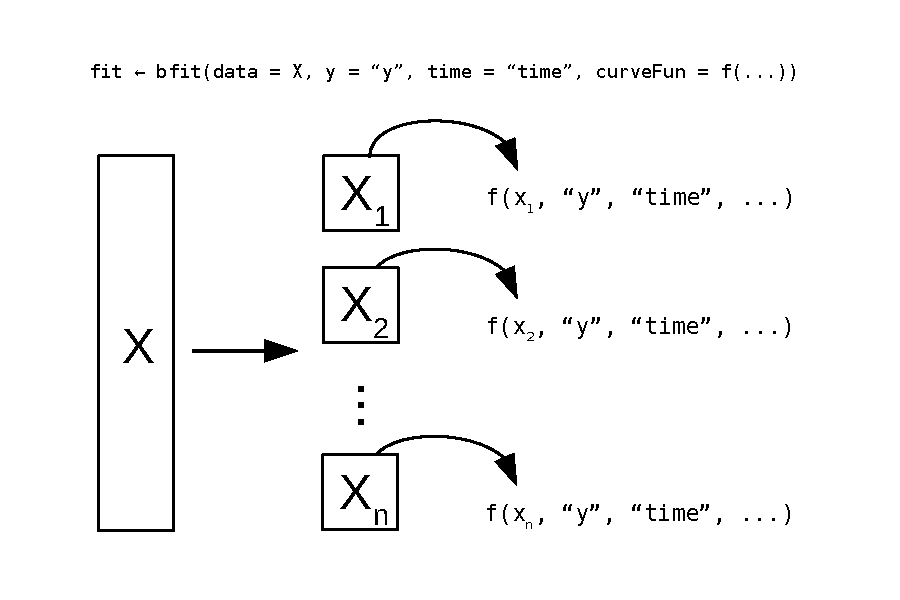
\includegraphics{img/curve_split.pdf}
\caption{A call to the function \xt{bfit} with data \xt{X} and outcome and time variables \xt{"y"} and \xt{"time"}. \xt{bfit} splits the dataset \xt{X} by subject/group and passes each individual \xt{data.frame} into the curve function \xt{f()}, along with time and outcome character vectors as well as any other arguments passed into \xt{`...`}. In particular, the \xt{`...`} argument allows the user to specify characteristics of the curve function that apply to all instances, as would be the case, for example, if \xt{curveFun = polynomial(degree = 5)}. Finally, each instance of \xt{f(...)} returns both a formula for \xt{lmer::gnls} as well as subject-specific starting parameters.}
\label{fig:curve_split}
\end{figure}

We turn our attention now to the curve function itself, using as an example a curve function for sitting a straight line to the observed data, given in Figure~\ref{fig:fun_layout}. In describing the purpose for each, we also include enough detail so that this may be used as a template in constructing a new one all together. We do this in an enumerated list, each item corresponding to the numbered portion in Figure~\ref{fig:fun_layout}.

\begin{figure}[H]
\centering
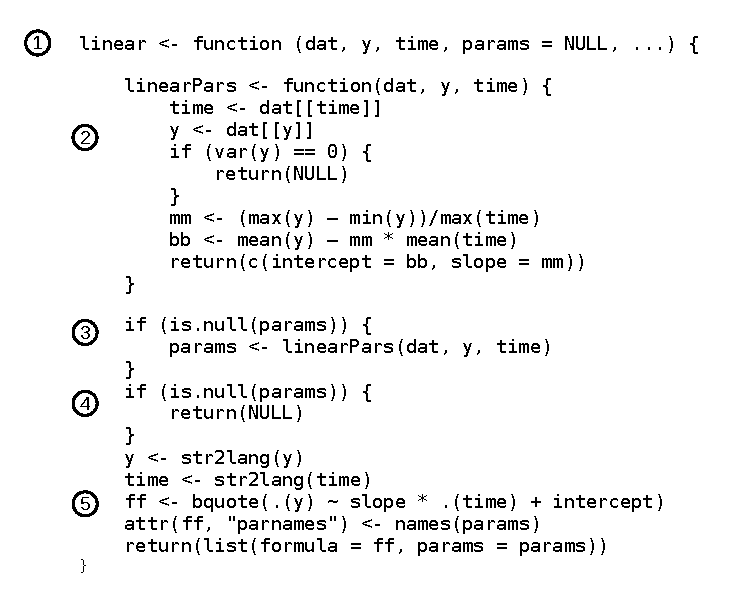
\includegraphics{img/fun_layout.pdf}
\caption{An example curve function with its constituent parts}
\label{fig:fun_layout}
\end{figure}

\begin{enumerate}
\item The first part of the curve function is the collection of arguments to be passed, also known as formals. Each curve function should have an argument \xt{dat}, which takes a \xt{data.frame} as described in Figure~\ref{fig:curve_split}, as well as arguments \xt{y} and \xt{time} which will take character strings indicating which columns of \xt{dat} represent the outcome and time variables, respectively. Following this is the prespecified argument \xt{params = NULL}, which is used by \xt{bdots} during the refitting process, where the estimated starting parameters for the function are retrieved from outside the curve fitting function. During the initial fitting process, however, these parameters are generally constructed from the observed data. The only exception to this would be if the user decided to specify the initial starting parameters for \emph{all} subjects when calling \xt{bfit}, as in the call

\begin{singlespace}
\begin{figure}[H]
\centering
\begin{BVerbatim}
fit <- bfit(dat, "y", "time", curveFun = linear(intercept = 0, slope = 1).
\end{BVerbatim}
%\caption{Illustration of Mouse data}
\end{figure}
\end{singlespace}
This should not be common. Following the \xt{params} argument, any other arguments specific to the curve function could be included. Although there are none for \xt{linear}, an example of when they might be used would be for \xt{polynomial}, in which the degree of the polynomial to be fit would be included. Finally, there is the \xt{...} argument, which is needed to accommodate the passing of any additional arguments from \xt{bfit} that are not a part of the curve function. Generally, this is not needed by the users but should be included nonetheless. 

\item Also included in a curve function is a second function to estimate starting parameters from the observed data. While not strictly necessary that it be included \textit{within} the curve function, it is useful for keeping the curve function self contained; parameter estimating functions defined outside of the curve function will otherwise still be used if they exist in the users calling environment. For estimating starting parameters for a linear function we see here the function \xt{linearPars}, taking as  its arguments \xt{dat}, \xt{y}, and \xt{time}. In this example, we check in case \xt{var(y) == 0}, which causes issues for \xt{lmer::gnls}, though in general it is a good idea to check for any other potential issues when estimating starting parameters (negative values for a logistic, for example). Importantly, this function returns a named vector, with the names of the parameters needing to match the parameter names in the formula given in (5). 
\item As detailed in (1), with the argument \xt{params = NULL}, the curve function should begin by estimating starting parameters. When different parameters are passed into \xt{params}, this is skipped.
\item This is a quick check on the result from (3). Had \xt{linearPars} returned a \xt{NULL} object, the curve function itself should return a \xt{NULL} object so that it is not passed to the fitter.
\item Finally, we have the most intricate part of the curve function, which is the construction of the formula object to be used by \xt{lmer::gnls}. The first two lines of this use the base R function \xt{str2lang} which turns a character string into an R language object (specifically, an unevaluated expression), making the names of the outcome and time variable suitable for a formula. The next line using the base R function \xt{bquote}. The function \xt{quote} returns its argument exactly as it was passed as an unevaluated expression; \xt{bquote} does the same but first substituting any of its elements wrapped in \xt{.()}. As it is written here, this will return a formula object using \xt{slope} and \xt{intercept} as is, but while replacing \xt{.(y)} and \xt{.(time)} with the appropriate names based on the column names in \xt{dat}. Finally, the names of the parameters are included as attributes to the formula object and the curve function concludes by returning a named list including both the formula object, as well as the named vector of parameters.
\end{enumerate}

The object returned by the curve function is not limited to just providing starting parameters for observed data; the formula itself is converted by \xt{bdots} into a function proper, capable of evaluating and bootstrapping values from that function in \xt{bboot}. And so long as a user is able to recreate the steps provided, they should be able to construct any sort of nonlinear function to be fit to their data, even if it is not included in \xt{bdots}.

While there is obvious utility in being able to specify \textit{new} curves for \xt{bdots} to fit, we describe a case here in which the flexibility of the curve function was used to recreate the \xt{doubleGauss()} function for use with our simulated data. In short, Chapter 3 details a proposed method for fitting data in the Visual World Paradigm relying \textit{not} on a densely sampled function in time, but rather as a collection of unordered binary observations. When the \xt{doubleGauss} function was originally introduced to \xt{bdots}, the empirically observed data was a relatively close match for its parametric form:

\begin{equation}
f(t|\theta) = \begin{cases}
\exp \left( \frac{(t - \mu)^2}{-2\sigma_1^2} \right) (p - b_1) + b_1 \quad \text{if } t \leq \mu \\
\exp \left( \frac{(t - \mu)^2}{-2\sigma_2^2} \right) (p - b_2) + b_2 \quad \text{if } t > \mu
\end{cases}
\end{equation}

An example of how the observed data matched the proposed functional form is taken from an example given in Figure~\ref{fig:bdots_log}.

\begin{figure}[H]
\centering
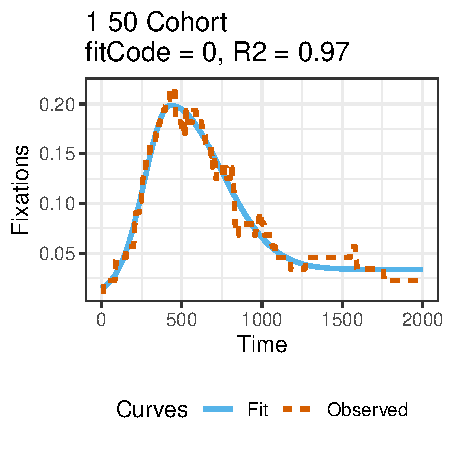
\includegraphics[scale=1]{img/bdots_logistic.pdf}
\caption{Observed data matching the parametric form of the asymmetrical Gaussian}
\label{fig:bdots_log}
\end{figure}

Accordingly, an appropriate function for estimating the starting parameters took the form given in Figure~\ref{fig:gauss_form}.


\begin{singlespace}
\begin{figure}[H]
\centering
\begin{BVerbatim}
dGaussPars <- function (dat, y, time) {
    time <- dat[[time]]
    y <- dat[[y]]
    if (var(y) == 0) {
        return(NULL)
    }
    mu <- time[which.max(y)]
    ht <- max(y)
    base1 <- min(y[time < mu])
    base2 <- min(y[time > mu])
    y1 <- y - base1
    y1 <- rev(y1[time <= mu])
    time1 <- rev(time[time <= mu])
    totalY1 <- sum(y1)
    sigma1 <- mu - time1[which.min(abs((pnorm(1) - pnorm(-1)) * 
        totalY1 - cumsum(y1)))]
    y2 <- y - base2
    y2 <- y2[time >= mu]
    time2 <- time[time >= mu]
    totalY2 <- sum(y2)
    sigma2 <- time2[which.min(abs((pnorm(1) - pnorm(-1)) * totalY2 - 
        cumsum(y2)))] - mu
    return(c(mu = mu, ht = ht, sig1 = sigma1, sig2 = sigma2, 
        base1 = base1, base2 = base2))
}
\end{BVerbatim}
\caption{Estimate starting parameters for empirical asymmetric Gaussian}
\label{fig:gauss_form}
\end{figure}
\end{singlespace}

This is appropriate, for example, when considering that the \xt{mu} parameter is estimated by finding \textit{when} the observed data is at its peak, while the \xt{ht} parameter is found to be the peak itself. In the case of the look onset method, however, data consists of non-ordered binary observations $\{0,1\}$ in time, making estimates for even these two parameters completely unreliable. An immediate consequence of this was that in a simulation of 1,000 subjects fit with asymmetric Gaussian data was conducted, less than half were able to return adequate fits from \xt{bdots}, proving problematic for any kind of systematic analysis in assessing the proposed method.

The solution was to provide a new curve function utilizing a different internal function for estimating starting parameters. The particular interest in presenting this here is how broad of a solution this may be to any number of problems: rather than attempting to construct parameters directly from the data (which may be misbehaved), we provide a reasonable distribution of starting parameters, drawing any number of samples from it, and retaining those which best fit the observed data:

\begin{singlespace}
\begin{figure}[H]
\centering
\begin{BVerbatim}
dgaussPars_dist <- function(dat, y, time, startSamp = 8) {
        time <- dat[[time]]
        y <- dat[[y]]
        
        if (var(y) == 0) {
            return(NULL)
        }
        
        spars <- data.table(param = c("mu", "ht", "sig1", "sig2", "base1", "base2"),
                            mean = c(630, 0.18, 130, 250, 0.05, 0.05), 
                            sd = c(77, 0.05, 30, 120, 0.015, 0.015), 
                            min = c(300, 0.05, 50, 50, 0, 0), 
                            max = c(1300, 0.35, 250, 400, 0.15, 0.15))
        
        fn <- function(p, t) {
            lhs <- (t < p[1]) * ((p[2] - p[5]) * 
                      exp((t - p[1])^2/(-2 * p[3]^2)) + p[5])
            rhs <- (t >= p[1]) * ((p[2] - p[6]) * 
                      exp((t - p[1])^2/(-2 * p[4]^2)) + p[6])
            lhs + rhs
        }
        npars <- vector("list", length = startSamp)
        for (i in seq_len(startSamp)) {
            maxFix <- Inf
            while (maxFix > 1) {
                npars[[i]] <- Inf
                while (any(spars[, npars[[i]] <= min | npars[[i]] >= max])) {
                  npars[[i]] <- spars[, rnorm(length(npars[[i]])) * sd + mean]
                }
                maxFix <- max(fn(npars[[i]], time))
            }
        }
        r2 <- vector("numeric", length = startSamp)
        for (i in seq_len(startSamp)) {
            yhat <- fn(npars[[i]], time)
            r2[i] <- mean((y - yhat)^2)
        }
        finalPars <- npars[[which.min(r2)]]
        names(finalPars) <- c("mu", "ht", "sig1", "sig2", "base1", "base2")
        return(finalPars)
    }
\end{BVerbatim}
\caption{Using random distribution to estimate starting parameters}
\label{fig:gauss_form_dist}
\end{figure}
\end{singlespace}

By utilizing an existing fitting function while substituting the method by which the starting parameters are estimated, we were able to go from recovering less than half of the simulated starting parameters successfully to well over 80\%.



